\section{Per-Problem Mode Router: Honest Negative}
\label{sec:mode_router}

The discussion of future work in \S\ref{sec:discussion} sketches a
``Paper 2'' direction in which a learned router selects per-input
between mode-specific configurations.  A natural starting point is
the offline-replay form of that router: given the all-conditions
sweep over a fixed problem set, can a contextual classifier with
per-problem features pick the right condition for each problem and
beat the best fixed condition?  This section reports the Phase-2
attempt at that question, and the answer at our budget is no.  We
include the result here rather than in the discussion because the
pathology is structurally parallel to the verifier-aggregation
negative in \S\ref{sec:voting_gap}: at small $N$ with a large action
space and surface text features, supervised classification cannot
recover the oracle ceiling, regardless of whether the classification
target is per-branch correctness or per-problem condition.

\subsection{Setup}
\label{subsec:mode_router_setup}

The substrate is a $20$-problem $\times$ $12$-condition full
coverage of the public showcase examples.  The twelve conditions
span the AR-only baseline (\code{c1}), the LLaDA-only baselines
(\code{c2}, \code{c2c}, \code{c2hint}, \code{c2empty}), the AR-plan
$\to$ LLaDA pipelines (\code{c3}, \code{c3p}, \code{c4},
\code{cmerge}, \code{crev}), and the branch-aggregation conditions
(\code{cmaj}, \code{cmajc}).  Per-problem features are
question length, count of numeric tokens, and unigram/bigram TF-IDF
over the question text.  The classifier head is logistic regression
or random forest, trained leave-one-problem-out cross-validation
(LOOCV) with class weights balanced.

The pre-registered decision rule was $\geq 80\%$ LOOCV accuracy
beats the best-fixed baseline; below that, LOSS.

\subsection{Result: $-10$\,pp vs Best Fixed}
\label{subsec:mode_router_result}

\begin{table}[h]
\centering
\caption{Per-problem mode-router accuracy on the $20$-problem
$\times$ $12$-condition substrate, LOOCV.  The best fixed baseline
(\code{c2empty}, also matched by \code{cmajc}) is $75\%$; the
oracle (any-condition-correct) is $85\%$.  Both bandit variants
underperform the best-fixed baseline by $10\text{--}15$\,pp.
Pre-registered LOSS threshold ($<80\%$) hit.}
\label{tab:mode_router}
\smallskip
\small
\begin{tabular}{lr}
\toprule
Setting & Accuracy on $20$ problems \\
\midrule
\code{c1} (Qwen-$0.5$B AR alone) & $25\%$ \\
\code{c2c} (LLaDA $+$ commit-LoRA) & $70\%$ \\
\code{cmaj} (LLaDA $b{=}5$ vote) & $65\%$ \\
\code{c2empty} (LLaDA $+$ empty prefix, best fixed) & $\mathbf{75\%}$ \\
\code{cmajc} (sfumato-v3 default) & $75\%$ \\
\midrule
\textbf{Oracle} (any-condition-correct) & $\mathbf{85\%}$ \\
\midrule
D1 logistic-regression bandit (LOOCV) & $65\%$ \\
D1 random-forest bandit (LOOCV) & $60\%$ \\
\midrule
$\Delta$ best bandit vs best fixed & $-10$\,pp \\
\bottomrule
\end{tabular}
\normalsize
\end{table}

The bandits choose the right condition fewer than three times in
five.  Action histograms show why: the LR bandit picks \code{c2}
($11/20$) and \code{c1} ($6/20$) on most folds, with only
$3/20$ folds reaching the harder ($\code{c2c}$, \code{c2empty})
conditions; class weights notwithstanding, the LOOCV folds expose a
single training problem per held-out fold and the policy collapses
to the modal-easy-correct condition.

The $-10$\,pp deficit relative to \code{c2empty} is large enough at
$N{=}20$ that the LOSS verdict survives any reasonable
binomial-error correction; at this substrate scale the offline-replay
form of D1 is dead.

\subsection{Same Pathology as the Voting-Rule Gap}
\label{subsec:mode_router_pathology}

The $20$-problem $\times$ $12$-action setting here mirrors the
$200$-problem $\times$ $5$-branch setting of
\S\ref{sec:voting_gap}.  Both ask supervised classification with
surface features (question text in this section, candidate-solution
text in \S\ref{sec:voting_gap}) to recover an oracle ceiling
(any-correct-condition-here, any-correct-branch-there).  Both
classifiers underperform the corresponding best fixed (best
condition here, majority vote there) by $9\text{--}15$\,pp.  In
both cases the bottleneck is the same: at this substrate scale,
surface features cannot distinguish setups in which the right
action will succeed from setups in which it will fail, because the
distinction lives in the branch's or problem's
\emph{problem-comprehension trajectory} rather than in its surface
form.  The frontier-judge positive control in
\S\ref{subsec:frontier_judge} is the converse demonstration: a
verifier whose internal reasoning matches or exceeds the
generator's recovers the gap, because the bottleneck is reasoning,
not classification.

We report this here because the parallel between the two negatives
hardens the diagnosis.  The path forward in both cases is the same
three options: a substantially larger encoder, a process-reward
verifier consuming per-step trajectory features, or step-level
human supervision.  Sub-block-level routing (the original D1
proposal: route on per-sub-block trajectory features rather than
per-problem text features) requires Workstream-C STATUS-schema
trace data that is not yet collected at the scale this section
would need.  \S\ref{subsec:mode_router_pre_scale} reports two
\$0 pre-scale audits that further narrow this leg of the
follow-up.

\subsection{Pre-Scale Audit: Per-Sub-Block Divergence (E2) and Feature Signal (G)}
\label{subsec:mode_router_pre_scale}

Before committing the trace-collection budget that a per-sub-block
trajectory-feature router would require, we ran two cheap
audits on existing artifacts to test the precondition that such a
router needs: a meaningful decision point at some sub-block
boundary $s \geq 1$ where (i) branches diverge and (ii) trajectory
features carry signal about which branch will be correct.  Both
audits are pure analysis on already-collected JSONL substrates;
zero new GPU spend.

\paragraph{E2 --- branch-divergence histogram.}  On the
$200$-problem \cmaj{} $b{=}5$ substrate
(\code{e4/results/raw\_cmaj\_k64\_seed0\_b5\_v3LoRA\_N200.jsonl},
the same substrate as \S\ref{sec:voting_gap}), we restrict to
the $108$ problems where the five branches disagree on the
extracted answer ($54\%$ of $N=200$).  For each problem we
re-tokenise each of the five branches with the \LLaDA{} tokenizer,
pad to the $128$-token generation length, and split into four
sub-blocks of $32$ tokens.  For every sub-block we compute the
pairwise token-level Levenshtein distance over all $10$ branch
pairs and mark the sub-block as ``diverged'' if any pair exceeds
edit-distance $3$.  First-divergence-sub-block is the smallest
diverged $s$.  As a cross-check, the same procedure run over
detokenised sub-block text with $1$-$2$gram TF-IDF cosine $\leq 0.7$
agrees with the token-level result on $95.4\%$ of problems.

\begin{figure}[h]
\centering
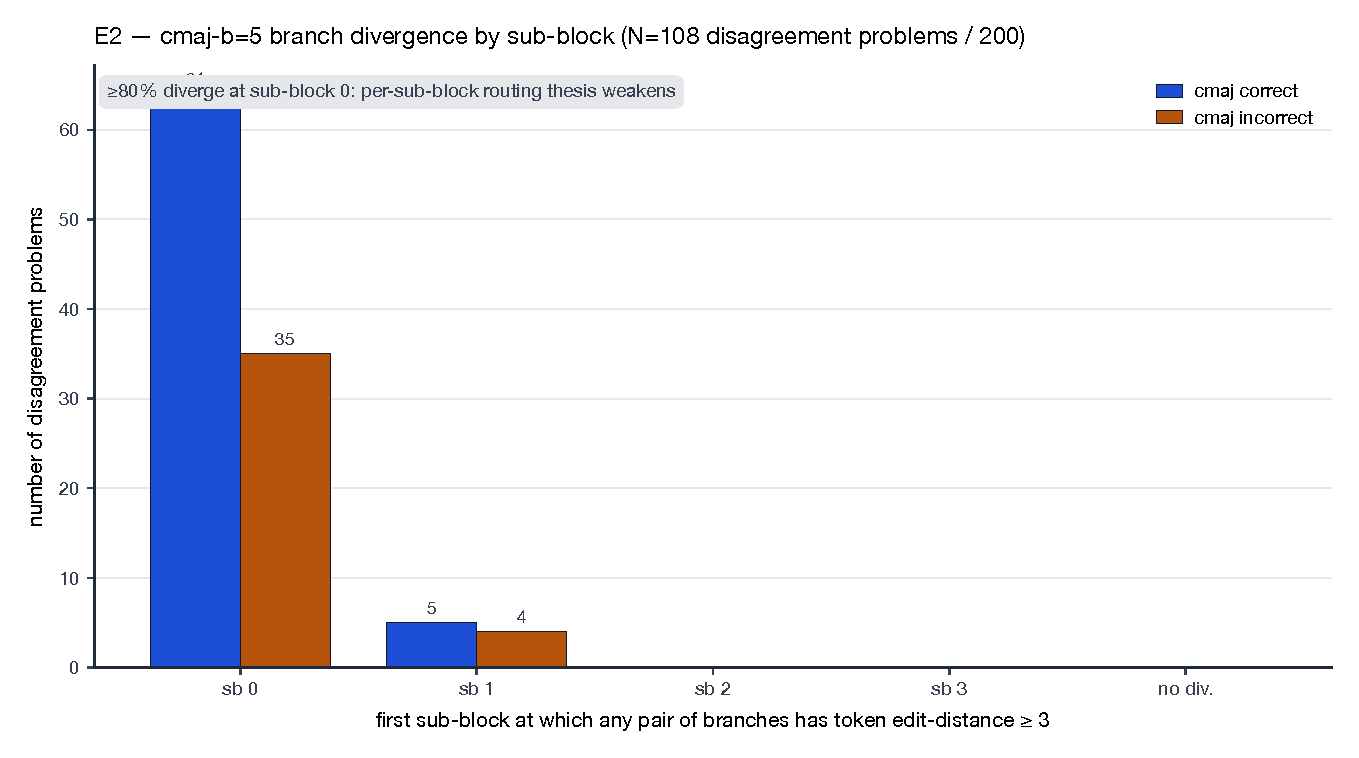
\includegraphics[width=0.92\textwidth]{figures/fig_e2_cmaj_divergence.pdf}
\caption{E2 --- where the five \cmaj{} branches first diverge,
stratified by \cmaj{}-correct vs \cmaj{}-incorrect, on the $108$
disagreement problems of the $N{=}200$ \cmaj{} $b{=}5$ substrate.
$91.7\%$ first diverge at sub-block~$0$ (the very first
$32$ generated tokens); $8.3\%$ first diverge at sub-block~$1$;
no problem first diverges at sub-blocks~$2$ or~$3$.  Semantic
TF-IDF cross-check returns $88.9\%$ at sub-block~$0$, agreeing
with the token-level result on $95.4\%$ of problems.}
\label{fig:e2_cmaj_divergence}
\end{figure}

The implication is sharp: at this substrate, branches that produce
different final answers have already chosen different problem
setups in their first $32$ committed tokens.  There is essentially
no mid-trajectory decision point ($s \geq 1$) for a per-sub-block
router to operate on.  The $\$0$ cost of E2 makes this an
inexpensive ratchet on what ``trajectory-feature routing at scale''
could possibly mean before any STATUS-schema collection runs.

\paragraph{G --- feature sanity check on the existing seven traces.}
A complementary precondition is whether trajectory features
predict correctness even at small $n$.  On the seven existing
Workstream-C deterministic traces
(\code{phase2/inference\_viz/traces/trace\_real\_p\{10..70\}\_*.jsonl})
we extract $17$ pooled trajectory features (mean / min / max /
std entropy; per-sub-block entropy at $s\in\{0,1,2,3\}$;
sub-block-$0$ min and max entropy; mean and sub-block-$0$ top-$k$
entropy; mechanism diversity; total and max wallclock;
commit-LoRA fraction; tokens-committed) and label each trace by
the correctness of its final extracted answer.  Univariate
Spearman~$\rho$ with $10{,}000$-permutation $p$-values gives one
feature passing the pre-registered $|\rho| \geq 0.5$ and
perm-$p \leq 0.10$ thresholds: \code{min\_entropy} with
$\rho{=}{-}0.79$, perm-$p{=}0.097$.  Three additional features
sit at $|\rho|{\approx}0.63$ but miss the $p$-threshold
($p{\approx}0.20$): \code{sb0\_entropy\_mean},
\code{sb0\_topk\_entropy\_mean}, \code{sb3\_entropy\_mean}.  All
sign-consistent: lower entropy predicts correct.  After
Bonferroni correction over $17$ features no individual feature
clears $0.05$, so the result is at best a $\textit{hint of
signal}$ at $n{=}7$, not an evaluation.  The strongest features
are sub-block-$0$ specific, consistent with E2.

\paragraph{Combined implication.}  E2 says branches diverge at
sub-block~$0$; G says any trajectory-feature signal is also
concentrated at sub-block~$0$.  A per-boundary router across
sub-blocks $0$--$3$ has empty inputs at $s \geq 1$ (no divergence
to condition on) and, if it could see the entire trajectory, would
key off sub-block-$0$ features.  The two viable architectures the
audits leave open are: (i) a problem-level pre-generation router,
which is the form already falsified in
\S\ref{subsec:mode_router_result} on $20$ problems with surface
text features (an open question is whether a sub-block-$0$
\emph{trajectory-feature} variant performs differently); and
(ii) a ``pilot-and-route'' architecture that runs a probe
sub-block~$0$, extracts trajectory features, and routes once
across the remaining $96$ tokens.  Per-boundary routing across
all four sub-blocks is empirically dead at this substrate.

The combined cost of E2 and G is \$0 (pure analysis on existing
JSONLs), and they tighten the ``follow-up work'' framing of
\S\ref{sec:discussion} from ``collect Workstream-C traces at
scale, see what works'' to ``test pilot-and-route specifically;
do not collect per-boundary trace data at scale for per-sub-block
routing''.

\subsection{What This Closes}
\label{subsec:mode_router_closes}

The original \code{sfumato/PLAN.md} listed a learned dynamic mode
router (E1) as a candidate headline contribution.  The result in
this section closes that thread as an honest negative at the
substrate scale we can afford.  In particular: the offline-replay,
per-problem, surface-text-feature form of D1 is not the
publishable mechanism.  The structural-separation argument for
mode routing in \S\ref{sec:discussion} (Future Work, ``Adaptive
mode router'') still stands at the design level; the empirical
realisation does not, at this scale and with this feature set.
A second honest negative --- a parameter-matched AR-only peer
baseline that beats the hybrid pipeline on this benchmark --- is
reported in the discussion (\S\ref{subsec:ar_baseline}).
